\section{Effect Of Aging On $\sigma_1'/\sigma_3'-\varepsilon$ Relationship 时效对$\sigma_1'/\sigma_3'-\varepsilon$关系的影响}

\begin{paracol}{2}
    
    In \autoref{figure:5a} and \autoref{figure:5b} are shown the variation of principal effective stress ratio with strain for samples consolidated isotropically and anisotropically, respectively.

    \switchcolumn

    在\cnsubfigureref{figure:5a}和\cnsubfigureref{figure:5b}中分别示出了各向同性和各向异性固结的样品的主要有效应力比随应变的变化。

    \switchcolumn*

    From the plotted curves it is observed at once that at a given strain the effective principal stress ratio is higher for samples with longer period of consolidation. However, the curves converge into a single one as the ratios approach their maximum value. This trend is observed for both the isotropically and the anisotropically consolidated samples, with the exception that the curve for samples consolidated anisotropically over a period of 4 months lies below the two others for large strains.

    \switchcolumn
       
    从绘制的曲线可以立即观察到,在给定应变下,固结时间较长的样品的有效主应力比较高。 但是,随着比率接近其最大值,曲线会收敛为一条曲线。 对于各向同性和各向异性固结的样品,都观察到了这种趋势,不同的是,在四个月的时间内,各向异性固结的样品的曲线低于大应变的两个曲线。

    \switchcolumn*

    The maximum values of $\sigma_1'/\sigma_3'$ are listed in \autoref{table:3} and they show no pronounced variation with the period of aging; if anything, there is a tendency towards a small reduction with aging.

    \switchcolumn
       
    \cntableref{table:3}中列出了$\sigma_1'/\sigma_3'$的最大值,并且它们没有显示出随老化时间的明显变化。 如果有的话,随着时间的流逝有减少的趋势。

\end{paracol}

\begin{figure}[!htbp]
    \centering
    \subfigure[CIU, tests on isotropically consolidated samples]{
        \label{figure:5a}
        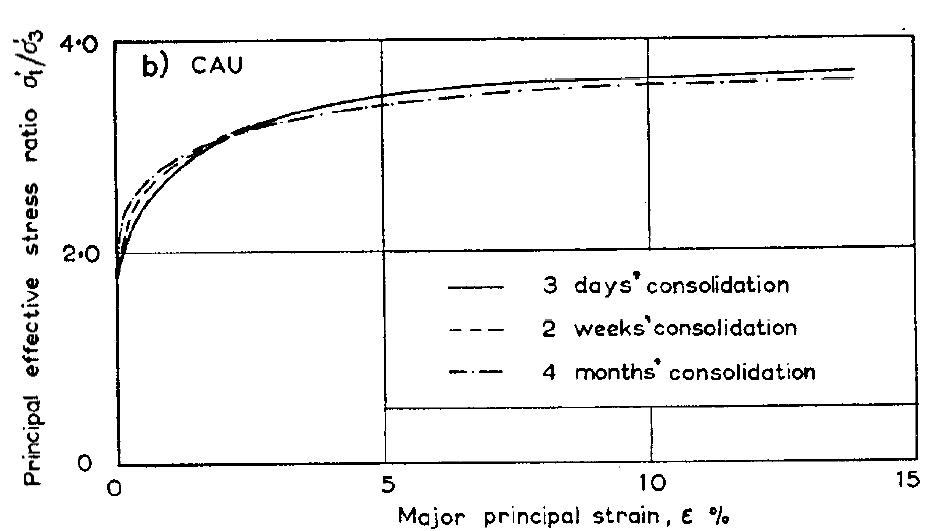
\includegraphics[width=0.48\textwidth]{figures/figure-5a.png}
    }
    \subfigure[CAU, tests on anisotropically consolidated samples]{
        \label{figure:5b}
        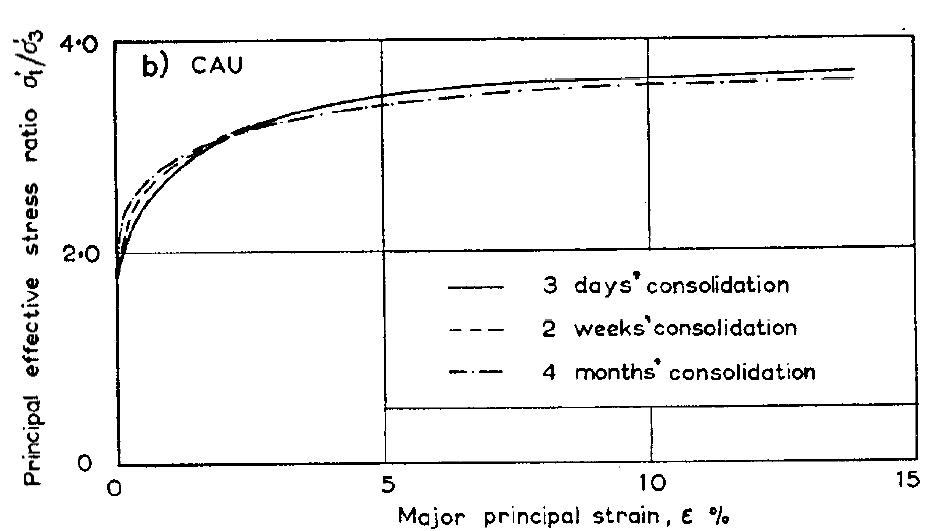
\includegraphics[width=0.48\textwidth]{figures/figure-5b.png}
    }
    \caption{Principal effective stress ratio as observed in consolidated undrained tests, Each curve represents the average of two tests.}
    \addtocounter{figure}{-1}
    \vspace{-5pt}
    \renewcommand{\figurename}{图}
    \caption{固结不排水试验中观察到的主要有效应力比,每条曲线代表两次试验的平均值。}
    \renewcommand{\figurename}{Figure}
    \label{figure:5}
\end{figure}